\section*{Приборы и принадлежности}

Лабораторный макет установки для
моделирования электростатического поля изображён на рис. \ref{fig:unit}.

В работе используется планшет 1, покрытый проводящей бумагой, с
нанесенными на него металлическими электродами 2. На планшете
установлены две подвижные линейки 3, с помощью которых определяются
координаты щупа 4, подключенного к вольтметру PV. Помещая щуп в разные
точки планшета и измеряя потенциал данной точки, можно построить
картину исследуемого поля. 


\begin{figure}[h]
	\centering
	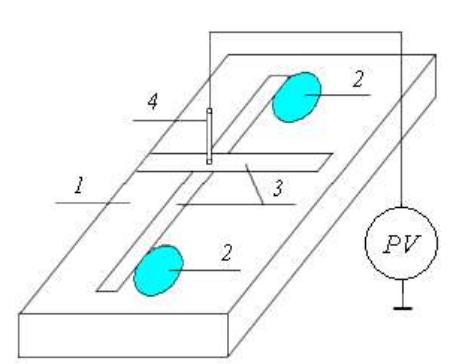
\includegraphics[width=0.6\linewidth]{photo/unit}
	\caption{Установка для моделирования электростатического поля}
	\label{fig:unit}
\end{figure}